\documentclass{article}
\usepackage[utf8]{inputenc}
\usepackage{amsmath}
\usepackage{layout}
\usepackage{float}
\usepackage{algorithm}
\usepackage{algorithmic}
\usepackage[shortlabels]{enumitem}
\usepackage{graphicx}
\setlength{\voffset}{-0.75in}
\setlength{\headsep}{5pt}
\setlength\parindent{0pt}
\usepackage{titling}
\renewcommand\maketitlehooka{\null\mbox{}\vfill}
\renewcommand\maketitlehookd{\vfill\null}

\graphicspath{./images/}

\title{Probabilistic Reasoning\\CS:440 Assignment 2}
\author{Christopher Naporlee - cmn134\\Michael Nelli - mrn73\\Timothy Walker - tpw32}
\date{April 2022}

\begin{document}
\maketitle
\newpage
\section*{Question 1}
\begin{enumerate}[a)]
    \item $P(A, B, C, D, E)$% 1a
    \begin{gather*}
        = P(D|A, B)P(E|B,C) P(A) P(B) P(C)\\
        = (0.1)(0.3)(0.2)(0.5)(0.8)\\
        = 0.0024
    \end{gather*}

    \item $P(\neg A,\neg B,\neg C,\neg D,\neg E)$% 1b
    \begin{gather*}
        = P(\neg D|\neg A,\neg B)P(\neg E|\neg B,\neg C) P(\neg A) P(\neg B) P(\neg C)\\
        = (1 - 0.9)(1 - 0.2)(1 - 0.2)(1 - 0.5)(1 - 0.8) \\
        = (0.1)(0.8)(0.8)(0.5)(0.2)\\
        = 0.0064
    \end{gather*}

    \item $P(\neg A | B,C,D,E)$
    \begin{gather*}
        = P(\neg A, B, C, D, E) \\
        = P(\neg A) P(B)P(C)\sum_{D}P(D|A,B)\sum_{E}P(E|B,C)
    \end{gather*}
    At this point we know that B and C are set to be true so we can easily derive
    the probability values for those. Also we can easily find E to be 0.3, because B, C are true.
    Finally, A is false and B is true thus D can only be 0.6.
    \begin{gather*}
        = (0.8)(0.5)(0.8)(0.3)(0.6) = 0.0576
    \end{gather*}
\end{enumerate}
\newpage

\section*{Question 2}
\begin{enumerate}[a)] % a), b), c), ...
    \item P(Burglary $|$ JohnCalls = True, MaryCalls = True)
    \begin{gather*}
        P(B | j,m) = \alpha P(B, j, m) \\
        = \alpha \sum_{e} \sum_{a} P(B, j, m, e, a) \\
        = \alpha \sum_{e} \sum_{a} P(B)P(e)P(A|B,e)P(j|a)P(m|a) \\
        = \alpha P(B)\sum_{e}P(e)\sum_{a}P(a|B,e)P(j|a)P(m|a) \\
        = \alpha \underbrace{P(B)}_{f_1(B)}
            \sum_{e}\underbrace{P(e)}_{f_2(E)}
            \sum_{a}\underbrace{P(a|B,e)}_{f_3(A, B, E)}
                \underbrace{P(j|a)}_{f_4(A)}
                \underbrace{P(m|a)}_{f_5(A)}\\
                \\
        f_6(B,E) = \sum_{a}f_3(A, B, E)\times f_4(A)\times f_5(A) \\
        = (f_3(a, B, E) \times f_4(a) \times f_5(a)) +
            (f_3(\neg a, B, E) \times f_4(\neg a) \times f_5(\neg a))
    \end{gather*}
    \begin{gather*}
        = (
        \begin{bmatrix}
            0.95 & 0.29 \\
            0.94 & 0.001
        \end{bmatrix}
        \times (0.9) \times (0.7)) + (
        \begin{bmatrix}
            0.05 & 0.71 \\
            0.06 & 0.999
        \end{bmatrix}
        + (0.05) \times (0.01))\\
        =
        \begin{bmatrix}
            0.598525 & 0.183055 \\
            0.592235 & 0.0011295
        \end{bmatrix}
    \end{gather*}
    \\
    Simplifying:
    \begin{gather*}
        P(B|j,m) = \alpha f_1(B) \times \sum_{e} f_2(E) \times f_6(B, E)\\
        f_7(B) = \sum_{e}f_2(E) \times f_6(B, E)\\
        f_7(B) = f_2(e) \times f_6(B, e) + f_2(\neg e) \times f_6(B, \neg e)
    \end{gather*}
    \begin{equation*}
        = ((.002) \times
        \begin{bmatrix}
            0.598582 \\
            0.183055
        \end{bmatrix})
        + ((.998) \times
        \begin{bmatrix}
            0.592235 \\
            0.0011295
        \end{bmatrix})
        = 
        \begin{bmatrix}
            0.59224 \\
            0.00149 \\
        \end{bmatrix}
    \end{equation*}
    \begin{gather*}
        P(B|j,m) = \alpha f_1(B) \times f_7(B) \\
        = \alpha
        \begin{bmatrix}
            0.001 \\
            0.999
        \end{bmatrix}
        \times
        \begin{bmatrix}
            0.59224 \\
            0.00149
        \end{bmatrix}\\
        \approx
        \begin{bmatrix}
            0.284 \\
            0.716
        \end{bmatrix}
    \end{gather*}
    
\newpage
    \item In our final equation we had $P(B|j,m) = \alpha f_1(B) \times f_7(B)$.
    \begin{gather*}
        f_7(B) = f_2(e) \times f_6(B, e) + f_2(\neg e) \times f_6(B, \neg e)\\
        f_6(B,E) = (f_3(a, B, E) \times f_4(a) \times f_5(a)) +
            (f_3(\neg a, B, E) \times f_4(\neg a) \times f_5(\neg a))
    \end{gather*}
    From $f_6(B, E)$ we got:
    \begin{gather*}
        f_7(B, E) = (
        \begin{bmatrix}
            0.95 & 0.29 \\
            0.94 & 0.001
        \end{bmatrix}
        \times (0.9) \times (0.7)) + (
        \begin{bmatrix}
            0.05 & 0.71 \\
            0.06 & 0.999
        \end{bmatrix}
        + (0.05) \times (0.01))
    \end{gather*}
    Which ends up resulting in 10 multiplications and 4 additions. This is because these
    operations are \textbf{pointwise}.\\
    Next, from $f_7(B)$ we got:
    \begin{gather*}
        = ((.002) \times
        \begin{bmatrix}
            0.598582 \\
            0.183055
        \end{bmatrix})
        + ((.998) \times
        \begin{bmatrix}
            0.592235 \\
            0.0011295
        \end{bmatrix})
    \end{gather*}
    which is another 4 multiplications and 2 additions. Finally our last step being:
    \begin{gather*}
        = \alpha
        \begin{bmatrix}
            0.001 \\
            0.999
        \end{bmatrix}
        \times
        \begin{bmatrix}
            0.59224 \\
            0.00149
        \end{bmatrix}
    \end{gather*}
    To solve this part: 2 more pointwise multiplications. Followed by 1 addition and 1 division 
    to solve $\alpha$. Finally doing 1 division to normalize. Bringing us to a grand total 
    of 16 multiplications, 7 additions, and 2 divisions or 25 total operations.\\
    \\
    As for enumeration we must:
    \begin{gather*}
        P(b | j, m) = \frac{P(b, j, m)}{P(b, j, m) + P(\neg b, j, m)}
    \end{gather*}
    Where
    \begin{gather*}
        P(b|j,m) = \alpha P(b)\sum_{e}\sum_{a}P(e)P(a|b,e)P(j|a)P(m|a)
    \end{gather*}
    In enumeration, we must do 3 multiplications over 2 values for each variable we are
    iterating over ($e, a$). Thus, 3 * 4 = 12 multiplications with 3 additions as part of
    the summations. Finally, one final multiplication using P(b) to get the result. Leaving
    us with 13 multiplications and 3 additions.\\
    However, we must calculate $P(\neg b, j, m)$ in order to get the alpha. Thus: we get
    16 operations + another 16 operations for 32 operations. Then another addition and division
    to apply our normalization.\\
    Leaving us with a grand total of 34 operations to solve enumeration.\\
    \\
    Comparing: variable elimination does (34 - 25) = 9 less operations.
    
\newpage
    \item First solving $P(X_1|X_n = true)$ using enumeration. We can represent the equation like:
    \[ 
    P(X_1 | X_n) = P(X_1)\sum_{X_2}\sum_{X_3} ... \sum_{X_{n-1}} P(X_2 | X_1) P(X_3|X_2) ... P(X_n|X_{n-1}) 
    \]
    In words, we must account for all the hidden variables in the bayesian network. In this problem, there are
    $n - 1$ hidden variables ($X_2 ... X_{n-1}$). Therefore, we must take into account $2^{n-1}$ entries. 
    Thus, our total work to be done using enumeration will be $O(2^{n-1})$ or more simply $O(2^{n})$.\\
    \\
    Next solving $P(X_1|X_n = true)$ using variable elimination. We have:
    \[
    P(X_1 | X_n) = P(X_1)\sum_{X_2}P(X_2 | X_1)\sum_{X_3}P(X_3|X_2) ... \sum_{X_{n-1}} P(X_n|X_{n-1})
    \]
    Variable elimination works by summing out the hidden variables that do not depend on the query:
    \begin{gather*}
    P(X_1 | X_n) = P(X_1)\sum_{X_2}P(X_2 | X_1)\sum_{X_3}P(X_3|X_2) ... \sum_{X_{n-2}} P(X_{n-3}|X_{n-2})f_1(X_{n-1})\\
    = P(X_1)\sum_{X_2}P(X_2 | X_1)\sum_{X_3}P(X_3|X_2) ... \sum_{X_{n-3}} P(X_{n-4}|X_{n-3})f_2(X_{n-2})\\
    ...
    \end{gather*}
    Therefore, using this method, we are able to not repeat work already done unlike variable enumeration.
    Further, since this network is a singly linked chain we can reference one of it's properties. 
    "The time and space complexity of exact inference in poly-trees is linear in the size of the network" 
    (Bayesian Networks and Exact Inference Notes, Pg. 5).\\
    Therefore, the amount of work done using this method will be $O(n)$.
\newpage
\end{enumerate}
\section*{Question 3}
\begin{enumerate}[a)]
    \item
    \begin{itemize}
        \item $P(d|c)$
            \begin{gather*}
               P(d|c) = \alpha P(d, c) \\
               = \alpha \sum_{a} \sum_{b} P(a)P(b)P(c|a, b)P(d|b,c)\\
               = \alpha \sum_{a} P(a) \sum_{b} P(b)P(c|a, b)P(d|b,c) \\
               = \alpha <0.3375, 0.1125> \\ = <0.75, 0.25>
            \end{gather*}
        From our coded sample tests of $P(d|c)$ we got: \\
        Rejection Sampling: $<0.74413, 0.25586>$ with \% Error $\approx 0.80\%$ \\
        Weighted Sampling: $<0.74606, 0.25393>$ with \% Error $\approx 0.53\%$
        \item $P(b|c)$
            \begin{gather*}
               P(b|c) = \alpha P(b, c) \\
               = \alpha \sum_{a} \sum_{d} P(a)P(b)P(c|a, b)P(d|b,c)\\
               = \alpha  P(b) \sum_{a} P(a) P(c|a, b) \sum_{d} P(d|b,c) \\
               = \alpha <0.45, 0> \\ = <1, 0>
            \end{gather*}
        From our coded sample tests of $P(b|c)$ we got: \\
        Rejection Sampling: $<1, 0>$ with \% Error $= 0\%$\\
        Weighted Sampling: $<1, 0>$ with \% Error $= 0\%$
        \item $P(d|\neg a, b)$
            \begin{gather*}
               P(d|~a, b) = \alpha P(d, ~a, b) \\
               = \alpha  \sum_{c} P(a)P(b)P(c|a, b)P(d|b,c)\\
               = \alpha P(a)P(b) \sum_{c} P(c|a, b)P(d|b,c)\\
               = \alpha <0.3825, 0.5175> \\ = <0.425, 0.575>
            \end{gather*}
        From our coded sample tests of $P(d|\neg a, b)$ we got: \\
        Rejection Sampling: $<0.42200, 0.57799>$ with \% Error $\approx 0.71\%$ \\
        Weighted Sampling: $<0.43604, 0.55295>$ with \% Error $\approx 2.50\%$
    \end{itemize}
    From our results we can see that our tests are very much similar to our expected probability.
    
    \newpage
    \item Sampling Graphs on $P(d|c)$\\
        \begin{figure}[H]
            \centering
            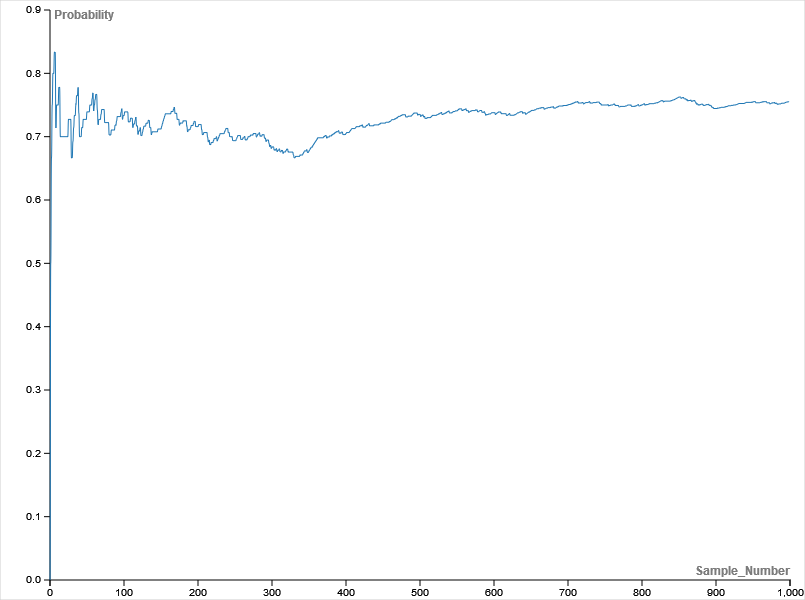
\includegraphics[width=\linewidth]{images/rejection_graph.png}
            \caption{Rejection Sampling on $P(d|c)$}
            \label{fig:rejection_graph}
        \end{figure}
        
        \begin{figure}[H]
            \centering
            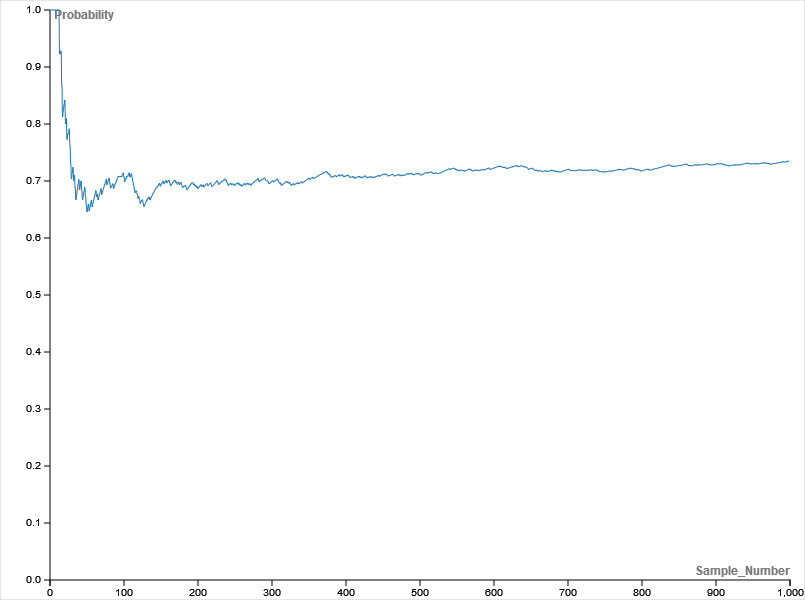
\includegraphics[width=\linewidth]{images/weighted_graph.png}
            \caption{Weighted Sampling on $P(d|c)$}
            \label{fig:weighted_graph}
        \end{figure}

        As you can see, the weighted sampling graph starts out not quite close to the expected probability,
        but levels out much quicker.
        As opposed to the rejection graph which starts closer to the expected probability, but fluctuates
        a lot more. This is because (if you look close enough) there are samples being rejected which cause
        it to take much longer to stabilize at our expected probability.
        
    \clearpage
    \item Our formulated query we used was: $P(d|\neg a,b, \neg c)$
        \begin{figure}[H]
            \centering
            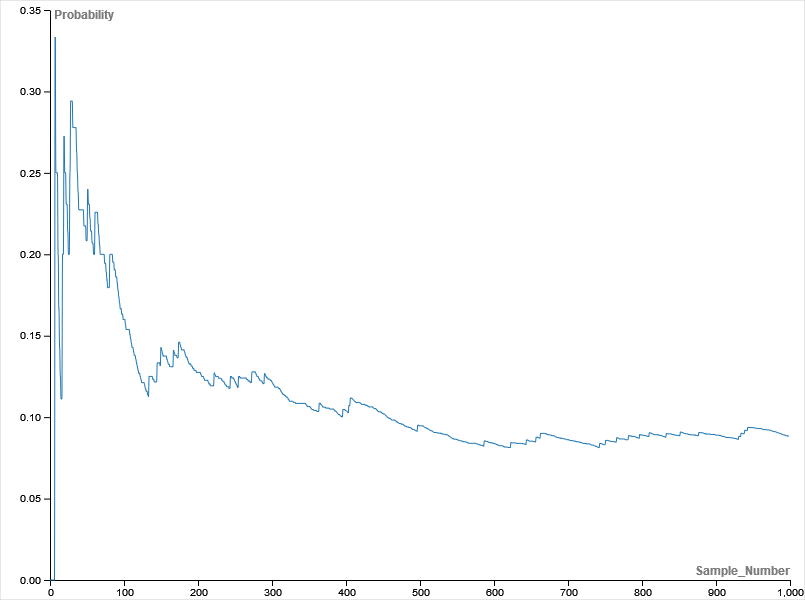
\includegraphics[width=\linewidth]{images/rejection_sampling_ourquery.png}
            \caption{Rejection Sampling on $P(d|\neg a,b, \neg c)$}
            \label{fig:newquery_rejection_graph}
        \end{figure}
        
        \begin{figure}[H]
            \centering
            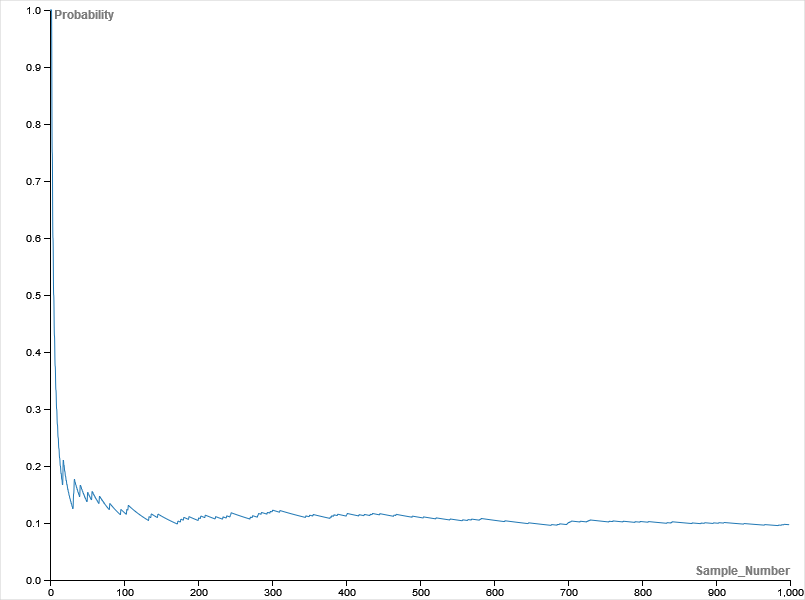
\includegraphics[width=\linewidth]{images/weighted_sampling_ourquery.png}
            \caption{Weighted Sampling on $P(d|\neg a,b, \neg c)$}
            \label{fig:newquery_weighted_graph}
        \end{figure}
        From these graphs, it is apparent that rejection sampling was notably worse. This is due
        to rejection samplings main pitfall - the fact that it will throw away too many samples.
        Given large amounts of evidence variables, as we have in our query of $\neg a, b, \neg c$, 
        rejection sampling will throw out a large amount of samples as it struggles to find the correct
        atomic event to validate as a matching sample.\\\\
        Knowing this, rejection sampling will need a much 
        larger set of samples in order to reach the expected probability output. As opposed to weighting, 
        that uses all the samples, it levels out much nicer and more quickly around 400 samples. 
        For rejection sampling, it has still yet to level out even at 400 samples.
\end{enumerate}

\clearpage
\section*{Question 4}
\begin{enumerate}[a)]
    \item Given: $X_1 = A$ Thus, $P(X_1 | hot_1) = 1$
    \begin{gather*}
        P(X_2 | hot_1, cold_2) \\
        = \alpha P(cold_2 | X_2) \sum_{X_1} P(X_2|X_1)P(X_1|hot_1)\\
        = \alpha <0, 1, 1, 0, 1, 1> \times <0.2, 0.8, 0, 0, 0, 0>\\
        = \alpha <0, 0.8, 0, 0, 0, 0> \\
        = <0, 1, 0, 0, 0, 0>
    \end{gather*}
    This answer makes sense, as if we were to start on A on day 1 and day 2 read cold we must have
    moved from A to B (a cold tile). Continuing...
    \begin{gather*}
        P(X_3|hot_1,cold_2,cold_3) \\
        = \alpha P(cold_3|X_3)\sum_{X_2}P(X_3|X_2)P(X_2|cold_2)
    \end{gather*}
    First we will solve for the summation:
    \begin{gather*}
        \sum_{X_2}P(X_3|X_2)P(X_2|cold_2) \\
        = [(<0.2, 0.8, 0, 0, 0, 0> \times 0) + (<0,0.2,0.8,0,0,0> \times 1) \\ 
            + (<0, 0, 0.2, 0.8, 0, 0> \times 0) + ...] \\
        = <0, 0.2, 0.8, 0, 0, 0>
    \end{gather*}
    Bring our answer back into the original equation:
    \begin{gather*}
        P(X_3 | hot_1, cold_2, cold_3) \\
        = \alpha P(cold_3 | X_3) <0, 0.2, 0.8, 0, 0, 0> \\
        = \alpha <0, 1, 1, 0, 1, 1> \times <0, 0.2, 0.8, 0, 0, 0>\\
        = \alpha <0, 0.2, 0.8, 0, 0, 0>\\
        = <0, 0.2, 0.8, 0, 0, 0>
    \end{gather*}
    Therefore, on the third day, we find that the probability of the rover being on B is 0.2, and
    the probability that it is on C is 0.8. Any other position has a probability of 0.
    
    \clearpage
    \item $P(X_2|hot_1,cold_2,cold_3)$
    \begin{gather*}
        = \alpha P(X_2 | hot_1, cold_2)P(cold_3|X_2) \\
        = \alpha <0, 1, 0, 0, 0, 0> \times P(cold_3 | X_2)
    \end{gather*}
    Solving for $P(cold_3|X_2)$:
    \begin{gather*}
        = \sum_{X_3}P(cold_3|x_3)P(|x_3)P(x_3|X_2)\\
        = (0 * 1 * <0.2, 0, 0, 0, 0, 0>) + \\
        (1 * 1 * <0.8, 0.2, 0, 0, 0, 0>) + \\
        (1 * 1 *  <0, 0.8, 0.2, 0, 0, 0 ,0>) +\\
        (0 * 1 * <0, 0, 0.8, 0.2, 0 ,0 ,0>) + \\
        (1 * 1 *  <0, 0, 0, 0.8, 0.2, 0>) + \\
        (1 * 1 *  <0, 0, 0, 0, 0.8, 0.2>) \\
        = <0.8, 1, 0.2, 0.8, 1, 0.2>
    \end{gather*}
    Back to the previous equation:
    \begin{gather*}
        \alpha <0, 1, 0, 0, 0, 0> \times P(cold_3 | X_2)\\
        = \alpha <0, 1, 0, 0, 0, 0> \times <0.8, 1, 0.2, 0.8, 1, 0.2>\\
        = \alpha <0, 1, 0, 0, 0, 0>\\ = <0, 1, 0, 0, 0, 0>
    \end{gather*}
    Thus,
    \[
        P(X_2|hot_1,cold_2,cold_3) = <0, 1, 0, 0, 0, 0>
    \]
    
    \clearpage
    \item Finding MLE given ($E_1=hot, E_2=cold, E_3=cold)$\\
    Our first point of explanation is given because we know the rover fell into A
    on the first day:
    \begin{gather*}
        V_1(X) = P(X_1) = <1, 0, 0, 0, 0, 0>\\
    \end{gather*}
    Next solving for day 2:
    \begin{gather*}
        V_2(X) = max_1[V_1(x_1)P(X_2|x_1)P(E_2 = cold | X_2)]\\
        = max[1 * 0.2 * 0, 1 * 0.8 * 1, 1 * 0 * 1, \ldots]\\
        = max[<0, 0.8, 0, 0, 0, 0>]\\
        = 0.8
    \end{gather*}
    That being that our most likely explanation for day 2 is that the rover went to B.
    Then, for day 3:
    \begin{gather*}
        V_3(X) = max_2[V_2(x_2)P(X_3|x_2) P(E_3 = cold | X_3)]\\
        =  max [0, 0.8 * 0.2 * 1, 0.8 * 0.8 * 1, 0 \ldots]\\
        = max [<0, 0.16, 0.64, 0, 0, 0>]\\
        = 0.64
    \end{gather*}
    From this we can gather that the rover most likely went to C on day 3.
    Therefore, our most likely explanation is:\\
    Day 1: $A$\\
    Day 2: $B$\\
    Day 3: $C$
    
    \clearpage
    \item $P(hot_4, hot_5, cold_6 | hot_1, cold_2, cold_3)$\\
        Given from previous information on the distribution of the rover to day 3, we know
        the rover must be on either B or C. Knowing this we can create paths that the rover
        could have taken.\\
        \begin{center}
        \begin{tabular}{|c|c|c|}
            \hline
            Starting Point Day 3 & Path & Probability \\
            \hline
            $B$ & $BBB$ & $\alpha 0.008$\\
            $B$ & $BBC$ & $\alpha 0.032$\\
            $B$ & $BCC$ & $\alpha 0.032$\\
            $B$ & $BCD$ & $\alpha 0.128$\\
            $B$ or $C$ & $CCC$ & $\alpha 0.008$\\
            $B$ or $C$ & $CCD$ & $\alpha 0.032$\\
            $B$ or $C$ & $CDD$ & $\alpha 0.032$\\
            $B$ or $C$ & $CDE$ & $\alpha 0.128$\\
            $C$ & $DDD$ & $\alpha 0.008$\\
            $C$ & $DDE$ & $\alpha 0.032$\\
            $C$ & $DEE$ & $\alpha 0.032$\\
            $C$ & $DEF$ & $\alpha 0.128$\\
            \hline
        \end{tabular}\\
        Where $\alpha = 1.666$
        \end{center}
        From this table, we can see that the ideal path for $hot_4, hot_5, cold_6$ given
        we are cold on day 3 is $DDE$ when starting on $C$.\\
        Therefore, 
        \[
            P(hot_4, hot_5, cold_6 | hot_1, cold_2, cold_3) = \alpha 0.032 = .0533
        \]
    \clearpage
    \item Solve $P(X_4|hot_1,cold_2,cold_3)$ and $P(X_5|hot_1,cold_2,cold_3)$
    \begin{gather*}
        P(X_4|hot_1,cold_2,cold_3)\\
        = \sum_{X_3}P(X_3|hot_1,cold_2,cold_3)P(X_4|X_3)
    \end{gather*}
    Solving for the summation first:
    \begin{gather*}
        \sum_{X_3}P(X_3|hot_1,cold_2,cold_3)\\
        = (0 * <0.2, 0.8, 0, 0, 0, 0>)\\
        + (0.2 * <0, 0.2, 0.8, 0, 0, 0>)\\
        + (0.8 * <0, 0, 0.2, 0.8, 0, 0>)\\
        + (0 * <0, 0, 0, 0.2, 0.8, 0>)\\
        + (0 * <0, 0, 0, 0, 0.2, 0.8>)\\
        + (0 * <0, 0, 0, 0, 0, 0.2>)\\
        = <0, 0.04, 0.32, 0.64, 0, 0>
    \end{gather*}
    Thus,
    \[
        P(X_4|hot_1,cold_2,cold_3) = <0, 0.04, 0.32, 0.64, 0, 0>
    \]
    
    Next, solving for $P(X_5|hot_1,cold_2,cold_3)$
    \begin{gather*}
        = \sum_{X_4}P(X_4|hot_1,cold_2,cold_3)P(X_5|X_4)\\
        = (0 * <0.2, 0.8, 0, 0, 0, 0>)\\
        + (0.04 * <0, 0.2, 0.8, 0, 0, 0>)\\
        + (0.32 * <0, 0, 0.2, 0.8, 0, 0>)\\
        + (0.64 * <0, 0, 0, 0.2, 0.8, 0>)\\
        + (0 * <0, 0, 0, 0, 0.2, 0.8>)\\
        + (0 * <0, 0, 0, 0, 0, 0.2>)\\
        = <0, 0.008, 0.096, 0.384, 0.512, 0>
    \end{gather*}
    Finally coming to:
    \[
        P(X_5|hot_1,cold_2,cold_3) = <0, 0.008, 0.096, 0.384, 0.512, 0>
    \]
\end{enumerate}

\newpage
\section*{Question 5}
\begin{enumerate}[a)]
    \item Finding $P(X_t | e, \alpha)$ where $\alpha$ denotes our action. Each matrix denotes
        the probability that we are at that position for each step. For full work, please
        check the included documents labeled "question5\_partA\_work" under the folder "q5".
    \begin{itemize}
        \item $P(X_1 | N, R)$
        \begin{gather*}
            = P(N|X_1)\sum_{X_0}P(X_1|X_0)P(X0|)\\
            =
            \begin{bmatrix}
                0.00131 & 0.01315 & 0.025 \\
                0.02368 & 0.2368 & 0.45 \\
                0.2368 &  & 0.013
            \end{bmatrix}
        \end{gather*}
        
        \item $P(X_2 | N, N, R)$
        \begin{gather*}
            = P(N|X_2)\sum_{X_1}P(X_2|X_1)P(X_1|N) \\
            =
            \begin{bmatrix}
                7.66*10^{-6} & 1.46 * 10^{-4} & 0.0021 \\
                0.0025 & 0.0474 & 0.698\\
                0.249 & & 7.6 * 10^{-4}
            \end{bmatrix}
        \end{gather*}
        
        \item $P(X_3 | N, N, H, D)$
        \begin{gather*}
            = P(H|X_3)\sum_{X_2}P(X_3|X_2)P(X_2|N, N)\\
            =
            \begin{bmatrix}
                1.78 * 10^{-6} & 2.247 * 10^{-5} & 1.796 * 10^{-5} \\
                2.198 * 10^{-5} & 0.00406 & 0.00613\\
                0.02148 & & 0.9682
            \end{bmatrix}
        \end{gather*}
        
        \item $P(X_4 | N, N, H, H, D)$
        \begin{gather*}
            = P(H|X_4)\sum{X_3}P(X_4|X_3)P(X_3|N, N, H) \\
            =
            \begin{bmatrix}
                1.825 * 10^{-7} & 2.304 * 10^{-6} & 1.023 * 10^{-7}\\
                2.165 * 10^{-7} & 2.324 * 10^{-4} & 3.583 * 10^{-5}\\
                0.00122 & & 0.9985
            \end{bmatrix}
        \end{gather*}
    \end{itemize}
    Given this information, we can conclude that we will have ended up in the bottom right of
    the map (3,3) with a probability of 0.9985.
    
    \item For example readings generated, please refer to the included python scripts and the
        files under the folder "q5" and the generated results under "results" within "q5".
    \clearpage
    \item \textbf{Filtering Visualizations}\\
        For the visualizations of the heat map, we created a program for you to interactively use.
        For relevant documentation read the README under 'q5' folder. As for the pictures, we have
        attached heatmaps for iterations 10, 50, and 100 along with the perceived action/sensors and
        the true actions. As for the meaning of the heat map:
        \begin{itemize}
            \item Grey cells represent a blocked cell with 0 probability.
            \item White cells represent a very low probability.
            \item Blue cells represent low/medium probability.
            \item Light red cells represent medium/high probability.
            \item Dark red cells represent an extremely high probability.
        \end{itemize}
\end{enumerate}
        \begin{figure}[H]
            \centering
            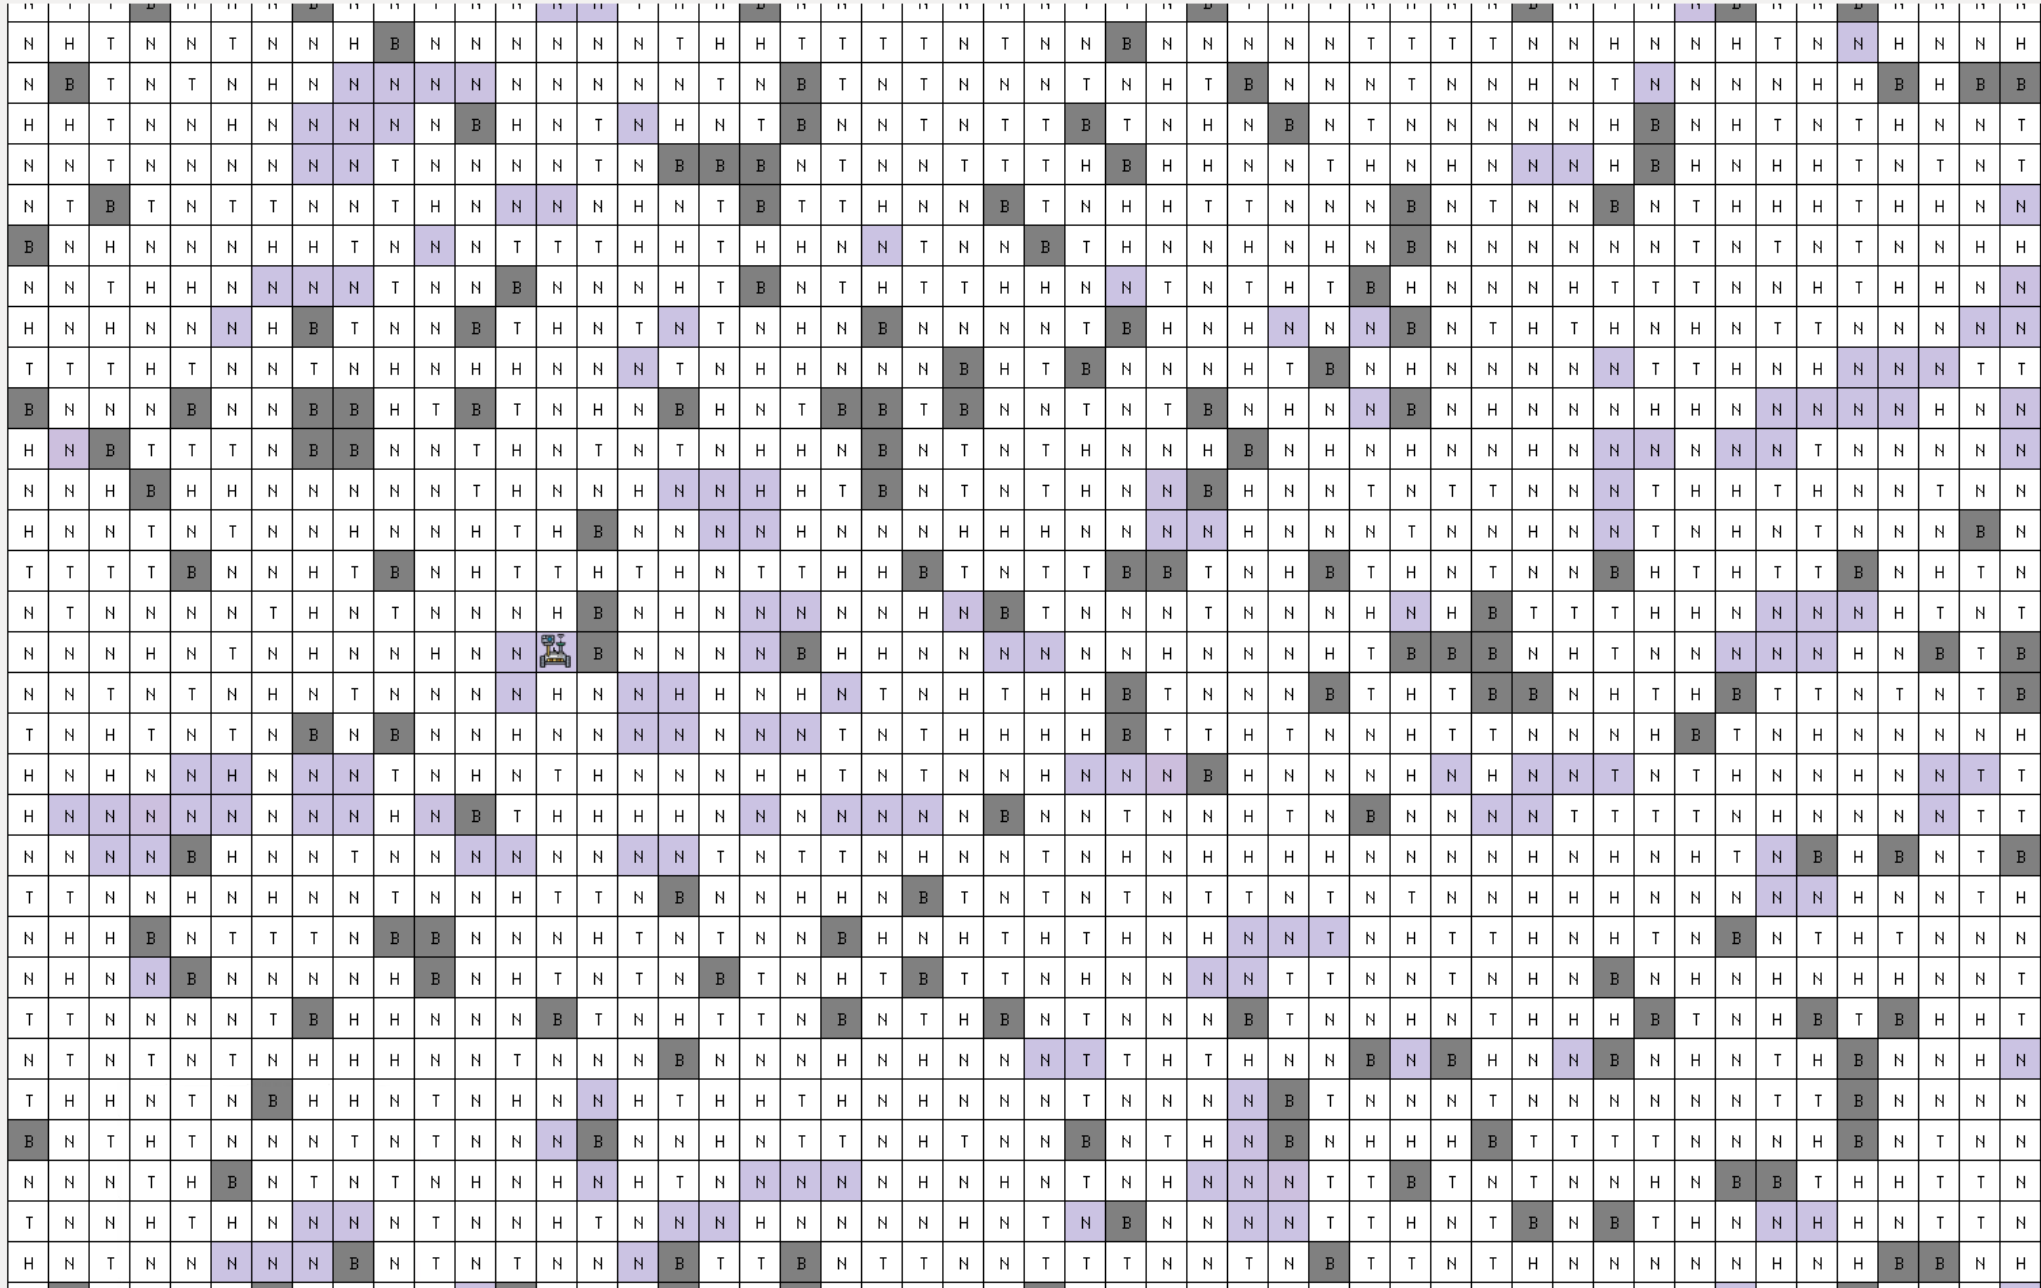
\includegraphics[scale=0.3]{images/10iter.png}
            \caption{Heatmap after 10 iterations.}
            \label{fig:heatmap_10iter}
            \small
            Actions: LLUDUDRURR\\
            Sensors: NNHNHNNNNN\\
            True Movement: LLUDUDRURR
        \end{figure}
        
        \begin{figure}[H]
            \centering
            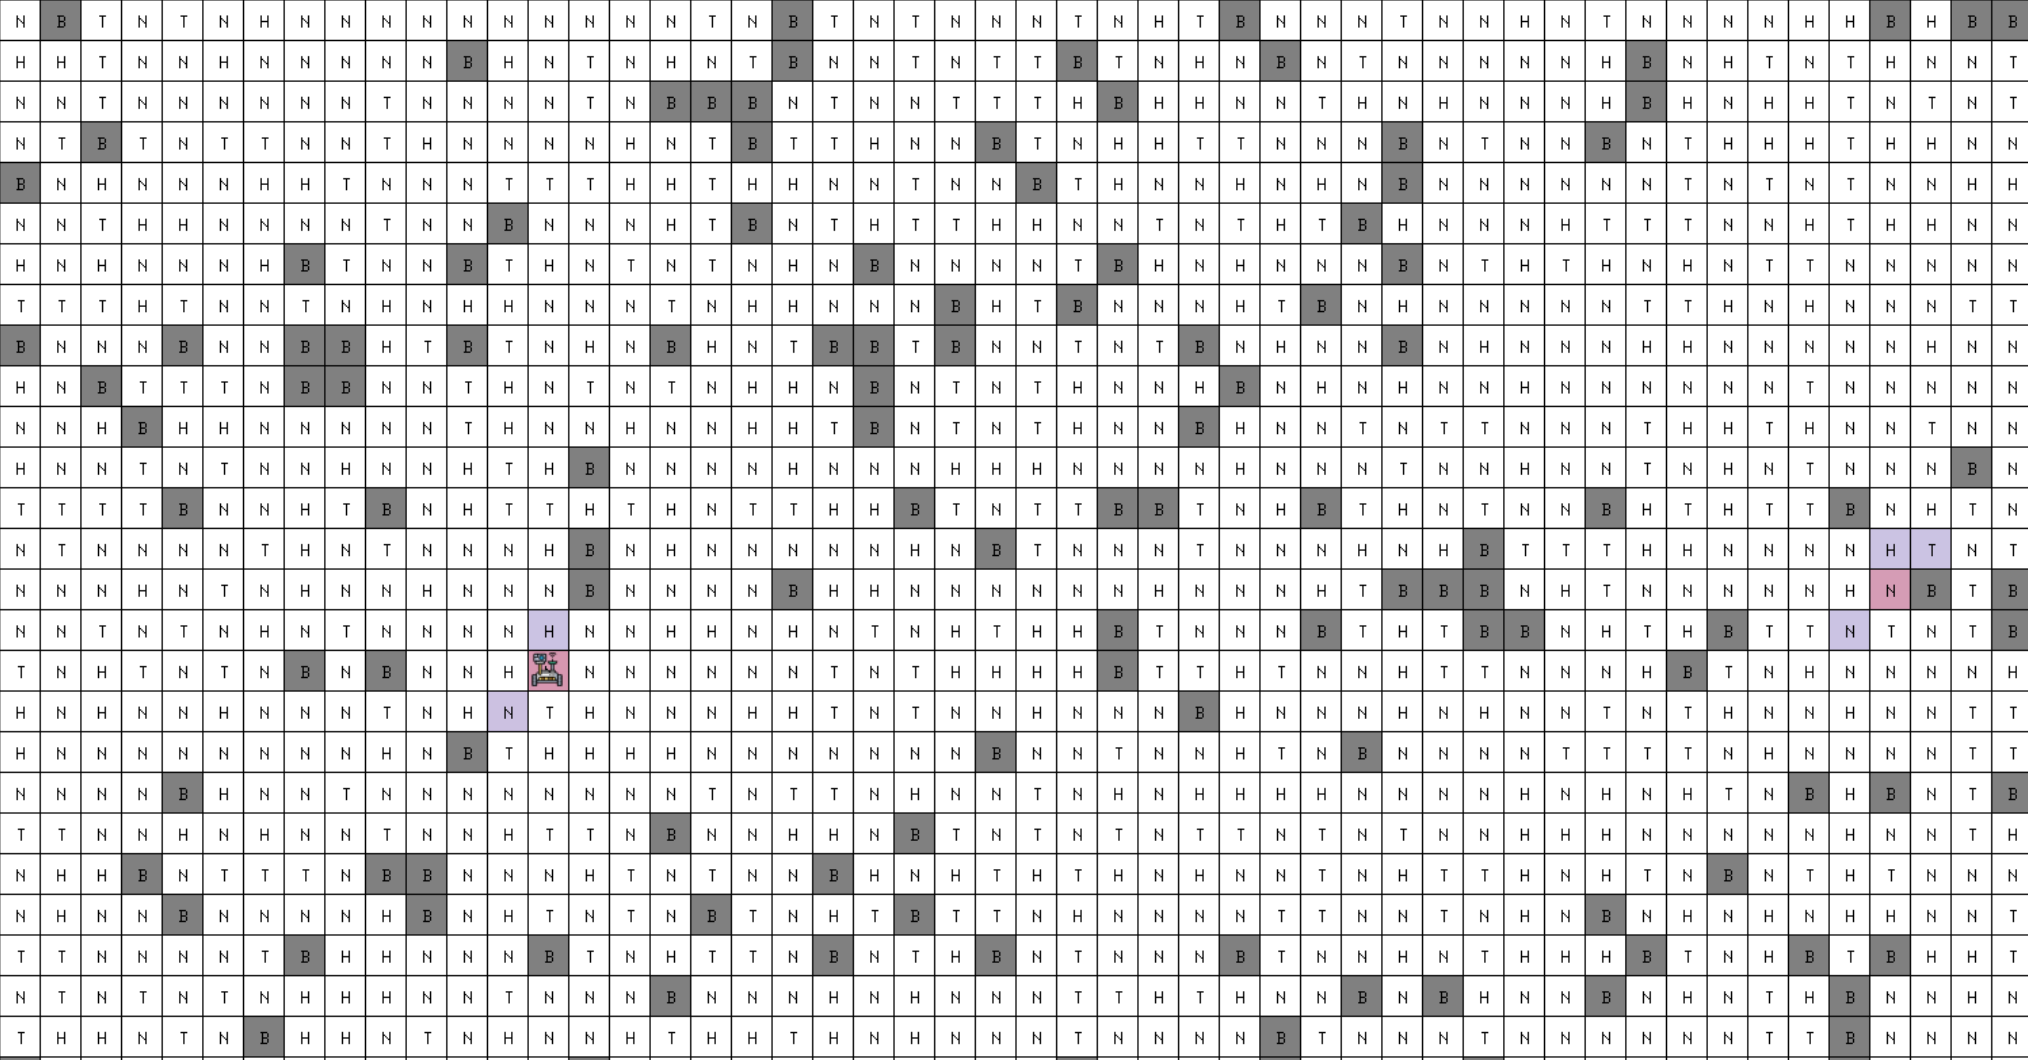
\includegraphics[scale=0.3]{images/50iter.png}
            \caption{Heatmap after 50 iterations}
            \label{fig:heatmap_50iter}
                    \small
                    Reported Actions:\\ LLUDUDRURRLDLRLLRDDLLLRLLRDDURDDDUUULRRUUDDRUUDRUD\\
                    Reported Sensors:\\ NNHNHNNNNNNNNNNNNHNHNTNTNHTNNNHNNNHNTNHNNHTNNHHNHN\\
                    True Movement (Dashes denote moments the rover stays still):\\
                        LLUDUDRURRLDLRL-RDDLLLRLLRDD--DDDUUULRR-UDDR-U-RUD
        \end{figure}
        
        \begin{figure}[H]
            \centering
            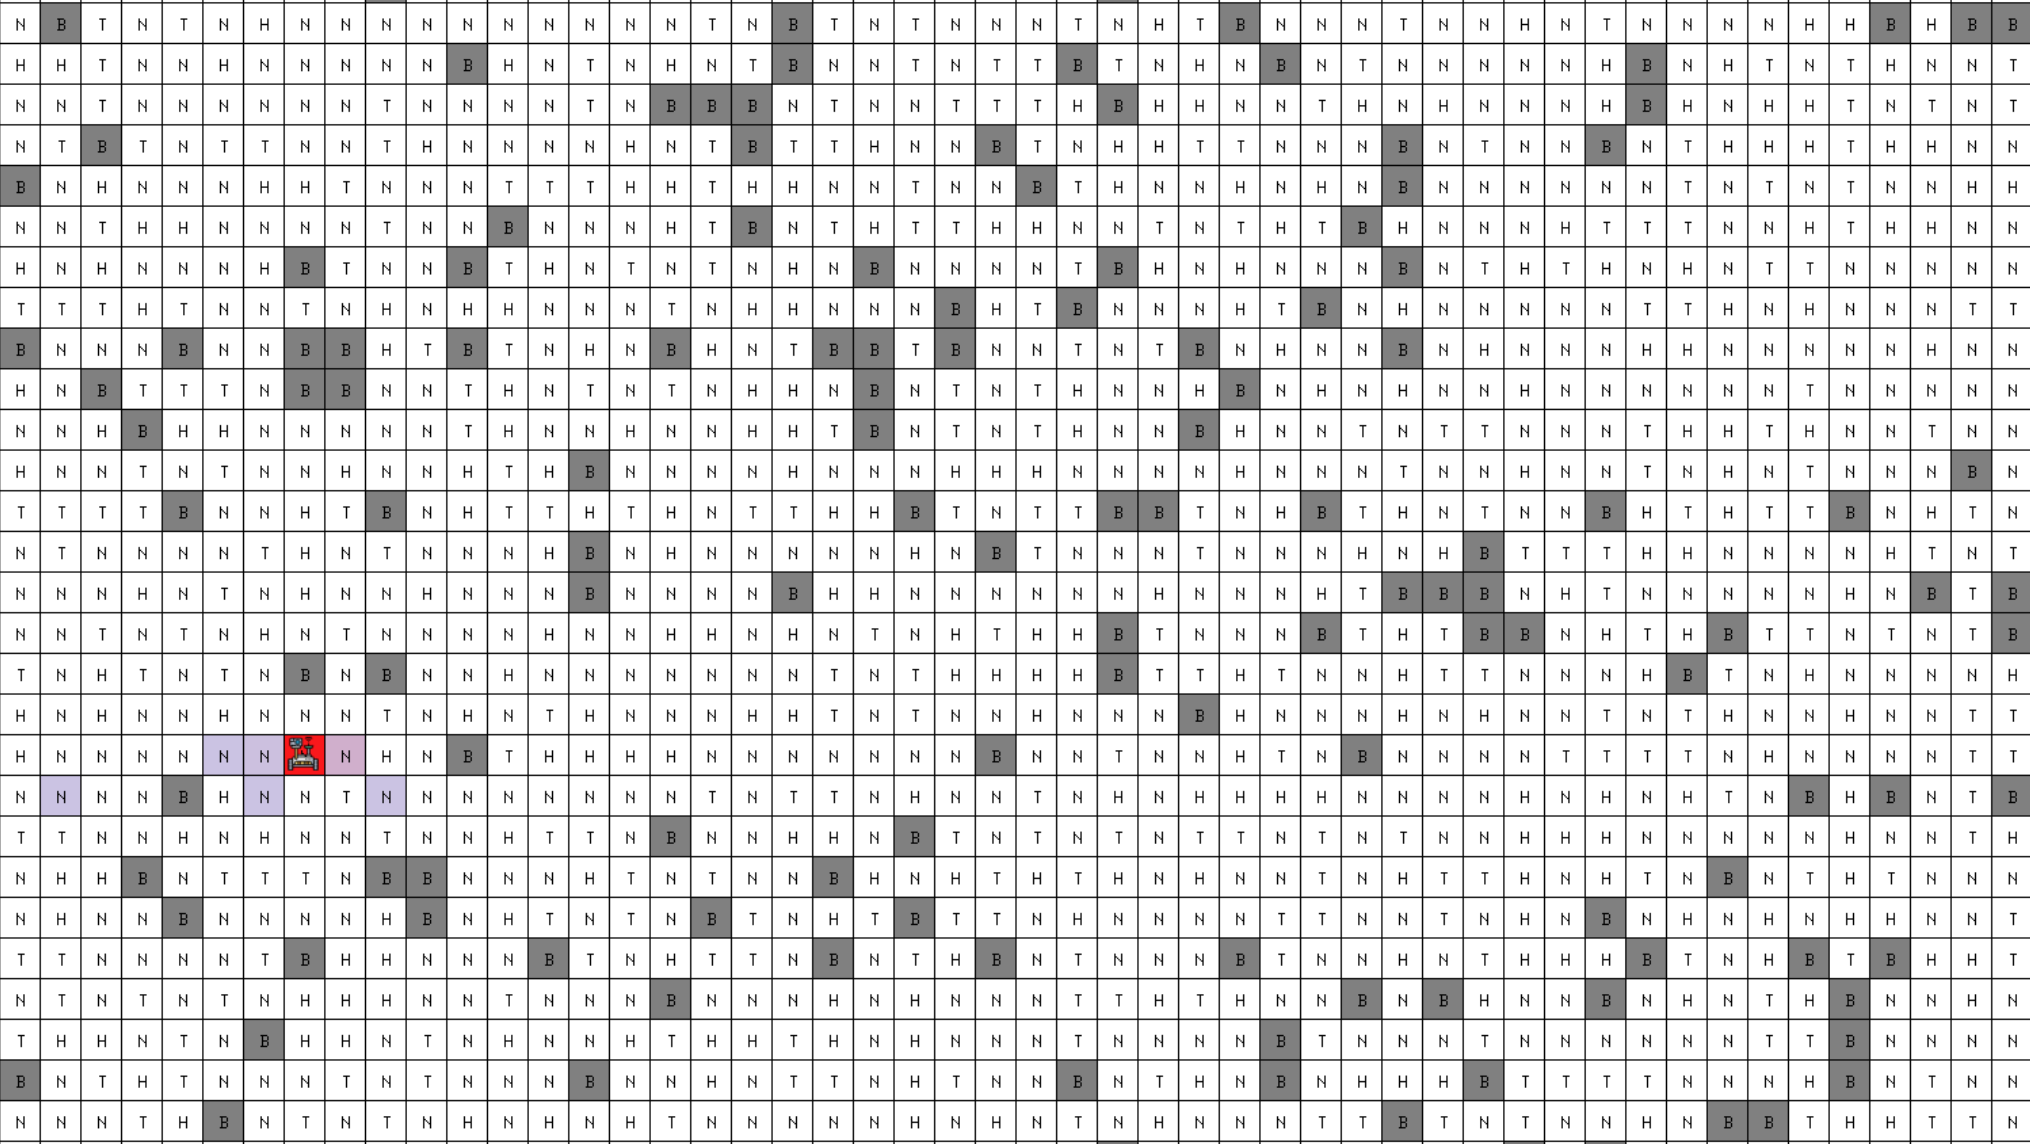
\includegraphics[scale=0.3]{images/100iter.png}
            \caption{Heatmap after 100 iterations}
            \label{fig:heatmap_100iter}
            \small
            Reported Actions:\\ 
                LLUDUDRURRLDLRLLRDDLLLRLLRDDURDDDUUULRRUUDDRUUDRUD\\
                DDDUDLDLLLURDDRLULDULLLDULUDRRDLLDLRLLLLRLRURRRLL\\
            Reported Sensors:\\
                NNHNHNNNNNNNNNNNNHNHNTNTNHTNNNHNNNHNTNHNNHTNNHHNHN\\
                THHTHTTNNNHNNNNNNHNHHNNHNNTNNNNNNNHNNHHNNHNNTNHNN\\
            True Movement (Dashes denote moments the rover stays still):\\
                LLUDUDRURRLDLRL-RDDLLLRLLRDD--DDDUUULRR-UDDR-U-RUD\\D-D-UDLDLLLURD-RLULDU-LLDULU-RRDLLDLR-LLLRLRURRRLL
        \end{figure}
        As you can see, by the 100th iteration, we are dark red on the cell that the agent is on. This
        deep red color denotes a probability of almost 1 meaning that our filtering algorithm is just 
        about certain that it is on that square.

        \clearpage
        \textbf{Plotting Error}\\
        \begin{figure}[H]
            \centering
            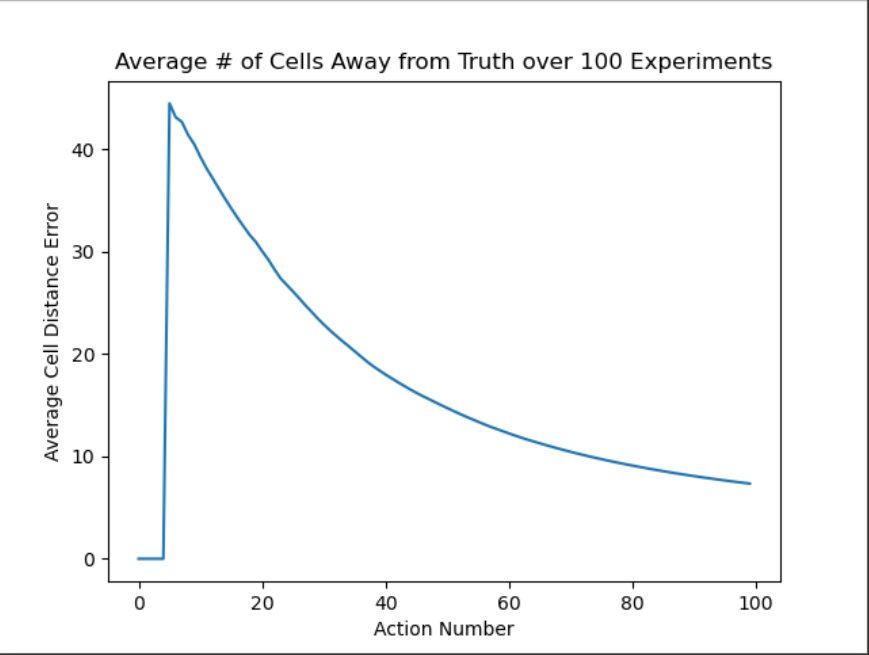
\includegraphics[width=\linewidth]{images/filter_err.png}
            \caption{Average number of cells off from true agent location for 100 actions 
                over 100 experiments with first 5 actions skipped.}
            \label{fig:filter_err}
            \small
        \end{figure}
        For plotting the error we found the number of cells away the max probability was from the true location
        of the agent for each action across each experiment. We took the average at each iteration across 100 
        experiments and got this plot. As you can see, as the number of actions increases the filtering algorithm
        gets closer and closer, on average, to the true location of the agent. 
        
        \clearpage
        \textbf{Agent Cell Probability}\\
        \begin{figure}[H]
            \centering
            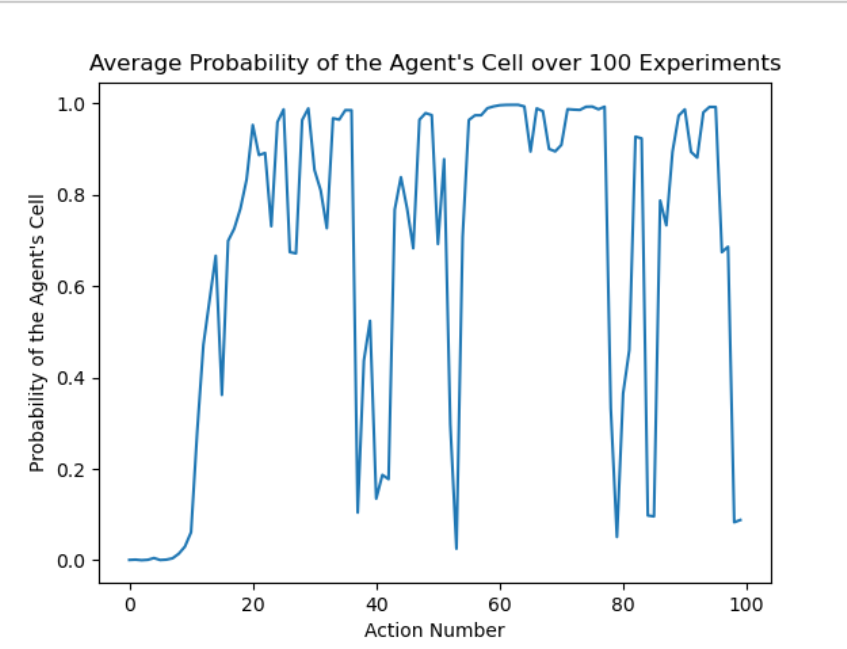
\includegraphics[width=\linewidth]{images/agent_cell_prob.png}
            \caption{Average Probability of Agent's Cell over 100 experiments}
            \label{fig:agent_prob}
            \small
        \end{figure}
        For plotting the probability of the agent's cell, we simply kept track of where he was in each experiment.
        Then, for each action we average the probability over 100 experiments. From the resulting graph we can see
        that for most of the time the filtering algorithm has a pretty good guess of where the agent truly is.
        However, we can also notice a lot of dips that indicate that the experiments have overlapping areas in
        which the agent reports one thing, but does another. Thus tricking the filtering algorithm into thinking
        the agent is somewhere else.

\newpage
\section*{Question 6}
\begin{enumerate}[a)]
    \item Expected net gain from buying $C_1$:
    \begin{itemize}
        \item \$4000 market value if in good shape
        \item \$3000 to buy
        \item \$1400 in repairs to make it in good shape (if not already)
        \item \$100 for mechanic test
        \item If in (70\% chance) good shape : (4000 - 3000) = \$1000 net profit
        \item If in (30\% chance) bad shape: (4000 - (3000 + 1400)) = -\$400 net profit
    \end{itemize}
    Net gain:
        \[ (0.7 * 1000) + (0.3 * -400) = \$580 \]
    \item
        \begin{gather*}
            P(pass(C_1)) = \sum_{q}P(pass(C_1) | q)\\
                    = P(pass(C_1) | q^+) P(q^+) + P(pass(C_1) | q^-) P(q^-)\\
                    = (0.8 * 0.7) + (0.35 * 0.3) \\= 0.665\\
            \\
            P(\neg Pass(C_1)) = 1 - P(pass(C_1)) = 1 - 0.665 = 0.335\\
        \end{gather*}
        Using this information we can find:
        \begin{gather*}
            P(q^+ | Pass) = \frac{P(Pass | q^+)P(q^+)}{P(Pass)} \approx 0.842\\
            \\
            P(q^+ | \neg Pass) = \frac{P(\neg Pass | q^+)P(q^+)}{P(\neg Pass)} \approx 0.418\\
            \\
            P(q^- | Pass) = 1 - P(q^+ | Pass) = 1 - 0.842 = 0.158\\
            \\
            P(q^- | \neg Pass) = 1 - P(q^+ | \neg Pass) = 1 - 0.418 = 0.582\\
        \end{gather*}
    \clearpage
    \item Using:
        \[ EU(A|E) = \sum_{i}P(Result_i(A) | Do(A), E) U(Result_i(A)) \]
    We can find:
        \begin{gather*}
            EU(buy | Pass) = \sum_{i}P(Result_i(buy) | Pass) U(Result_i(buy))\\
                = P(q^+ | Pass) U(q^+ | buy) + P(q^-,Pass)U(q^- | buy)\\
                = (0.842 * 1000) + (0.158 * -400) = 778.8\\
            \\
            EU(buy | \neg Pass) = \sum_{i}P(Result_i(buy) | \neg Pass) U(Result_i(buy)) \\
                = P(q^+ | \neg Pass) U(q^+ | buy) + P(q^-, \neg Pass)U(q^- | buy)\\
                = (0.418 * 1000) + (0.582 * -400) = 185.2\\
            \\
            EU(\neg buy | Pass) = \sum_{i}P(Result_i(\neg buy) | Pass) U(Result_i(\neg buy)) \\
                = P(q^+ | Pass) U(q^+ | \neg buy) + P(q^-,Pass)U(q^- | \neg buy)\\
                = (0.842 * 0) + (0.158 * 0) = 0\\
            \\
            EU(\neg buy | \neg Pass) = \sum_{i}P(Result_i(\neg buy) | \neg Pass) U(Result_i(\neg buy)) \\
                = P(q^+ | \neg Pass) U(q^+ | \neg buy) + P(q^-, \neg Pass)U(q^- | \neg buy)\\
                = (0.418 * 0) + (0.582 * 0) = 0
        \end{gather*}
        Therefore, the best decision given a pass is to buy, and the best decision 
            given a fail is to still buy.
    
    \clearpage
    \item Let the mechanic test be denoted by $T_j$.\\
    The value of perfect information is given by:
        \begin{gather*}
            VPI(T_j) = (\sum_{t_j}P(T_j=t_j)EU(\alpha_{t_j}|T_j=t_j)) - EU(\alpha)\\
                = [P(T_j = Pass) EU(\alpha_{Pass} | Pass) + P(T_j = \neg Pass) EU(\alpha_{\neg Pass} | \neg Pass)] - EU(\alpha)\\
                = [P(T_j = Pass) EU(buy | Pass) + P(T_j = \neg Pass) EU(buy | \neg Pass)] - EU(\alpha)\\
                = ((0.665 * 778.8) + (0.335 * 185.2)) - 580\\ 
                \approx -0.06
        \end{gather*}
    Therefore, you should not take $C_1$ to the mechanic as you will end up losing more money from it
    costing \$100.
\end{enumerate}

\newpage
\section*{Question 7}
For the following sections of information, it was all acquired from the code under the folder "q7".
    \begin{itemize}
        \item \textbf{Original Utilities}\\
            For our original utilities, we start with an array of 0's. As value iteration runs, 
            it will update this array. To understand this decision further refer to the algorithms
            written under the \textbf{implementation} section.
        \item \textbf{Intermediate Results}\\
            \begin{center}
            \begin{tabular}{|c|c|c|}
                \hline
                Iteration & Optimal Utilities $U$ & Policy $\pi$ \\
                \hline
                $1$ & $[0, 0, 0, 0]$ & $[1, 2, 3, 1]$\\
                $2$ & $[0, 0, 1.0, 0]$ & $ [1, 2, 3, 1]$\\
                $3$ & $[0, 0.72, 1.0, 0.81]$ & $[2, 2, 3, 1]$\\
                $20$ & $[3.2929, 3.7708, 4.3930, 3.8304]$ & $[2, 2, 3, 1]$\\
                $40$ & $[3.8516, 4.3366, 4.9499, 4.3972]$ & $[2, 2, 3, 1]$\\
                $60$ & $[3.9199, 4.4050, 5.0181, 4.4656]$ & $[2, 2, 3, 1]$\\
                $80$ & $[3.9282, 4.4133, 5.0264, 4.4739]$ & $[2, 2, 3, 1]$\\
                $100$ & $[3.9292, 4.4143, 5.0274, 4.4749]$ & $[2, 2, 3, 1]$\\
                $120$ & $[3.9293, 4.4144, 5.0276, 4.4751]$ & $[2, 2, 3, 1]$\\
                \hline
            \end{tabular}\\
            \textbf{Note:} For any $s_i$ the utility is $U[i - 1]$. Thus,
                the utility of $s_1$ is $U[1 - 1] = U[0]$. Similarly, for any $s_i$ the 
                policy is $\pi[i - 1]$. Thus, for the policy of $s_3$ the action to take is
                $\pi[3 - 1] = \pi[2] = 3 = a_3$ (for the 120$^{th}$ iteration).
            
            \end{center}
        \clearpage
        \item \textbf{Implementation}\\
            To calculate the optimal utilities and the optimal policy, we used the following algorithms
            and converted them to python code. We set our convergence criterion to be within
            5 decimal places or 0.00001.
            \begin{algorithm}
            \caption{Finding Optimal Utilities}
            \begin{algorithmic}
                \STATE \textbf{INPUTS:} Set of states $S$, transitional model $P(s'|s,a)$,
                    discount factor $\gamma$, and max error allowed in the utility of any state $\epsilon$
                \STATE \textbf{OUTPUT:} The optimal utilities $U$
                \STATE{}
                \STATE Initialize $U'$ to be array of zeros with length = $|S|$
                \WHILE{True}
                    \STATE $U \leftarrow U'$
                    \STATE $\delta \leftarrow 0$
                    \FOR{$s \in S$}
                        \STATE $U'[s] \leftarrow r(s) + \gamma max_a\sum_{s'}P(s'|s, a)U[s']$
                        \STATE $\delta \leftarrow max(\delta, |U'[s] - U[s]|)$
                    \ENDFOR
                    \IF{$\delta \leq \frac{\epsilon(1-\gamma)}{\gamma} $}
                        \STATE \textbf{break}
                    \ENDIF
                \ENDWHILE
                \STATE \textbf{return} $U$
            \end{algorithmic}
            \end{algorithm}
            
            \begin{algorithm}
            \caption{Finding Optimal Policy}
            \begin{algorithmic}
                \STATE \textbf{INPUTS:} Set of states $S$, transitional model $P(s'|s,a)$, and the
                    optimal utilities of each state $U$
                \STATE \textbf{OUTPUT:} The optimal policy $\pi^*$
                \STATE{}
                \STATE Initialize $\pi^*$ to be array of actions with length = $|S|$
                \FOR{$s \in S$}
                    \STATE $\pi^*(s) \leftarrow argmax_a\sum_{s'}P(s'|s, a)U[s']$
                \ENDFOR
                \STATE \textbf{return} $\pi^*$
            \end{algorithmic}
            \end{algorithm}
            These algorithms gave us a computation time: 0.113s over 124 iterations and our final result to be:\\
            $V_{opt} \approx [3.92937, 4.41448, 5.02761, 4.47512]$\\
            and\\
            $\pi^* = [2, 2, 3, 1]$\\
            \textbf{Note:} For any $s_i$ the utility is $U[i - 1]$. Thus,
                the utility of $s_1$ is $U[1 - 1] = U[0]$. Similarly, for any $s_i$ the 
                policy is $\pi[i - 1]$. Thus, for the policy of $s_4$ the action to take is
                $\pi[4 - 1] = \pi[3] = 1 = a_1$.
    \end{itemize}
\end{document}
